\documentclass[../main.tex]{subfiles}
\graphicspath{{\subfix{../images/}}, {\subfix{../diagrams/}}}

\begin{document}

    \chapter*{Introduzione}
    \addcontentsline{toc}{chapter}{Introduzione}
    	
        \section*{Il Contesto Aziendale}
        \addcontentsline{toc}{section}{Il Contesto Aziendale}
    	
    		\subsection*{Storia}
    		
    			\textbf{PerceptoLab S.r.l.} è una startup italiana (con seconda filiale in Germania) con sede a Giussano (MB), fondata nel 2017. L'azienda si è da sempre occupata di innovazione in ambito \emph{insurtech}, grazie a tecnologie proprietarie nell'ambito della \emph{Computer Vision} e dell'\emph{Intelligenza Artificiale}. Dal 2019 PerceptoLab si è concentrata sullo sviluppo dell'ecosistema \emph{Sphere}, una soluzione all-round per la gestione del \emph{claim} assicurativo e la digitalizzazione della propria abitazione. Il progetto consta inoltre di 2 brevetti depositati (Sphere Vision e Sphere Index).\\*
    			
    			L'azienda è ad oggi composta da 11 dipendenti, ad esclusione del \emph{CEO Dott. Mesiano Cristian}, divisi in 4 team diversi in base alla branca di lavoro: Mobile, Backend, Computer Vision e Deep Learning.
    		
    		\subsection*{Il progetto Sphere}
    		
    			In un mondo dove l'informazione risiede principalmente sotto forma di immagini, Sphere si propone come soluzione per trasformare il fisico in digitale, rompendo la barriera che divide una semplice fotografia da un elemento tangibile.
    			
    			\begin{figure}[H]
            		\centering
            		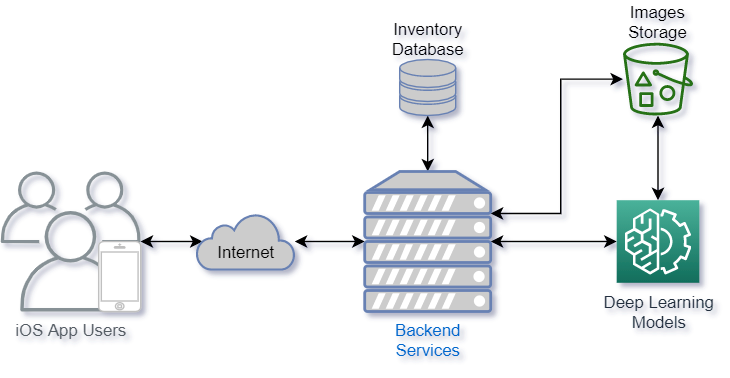
\includegraphics[width=0.7\textwidth]{sphere_base_arch}
            		\caption{Sphere - Architettura High Level}
            		\label{fig:sphere_base_arch}
        	    \end{figure}
    			
    			Grazie a Sphere\cite{plab_sphere} l'utente è in grado di creare un \emph{Digital Inventory} di casa propria, partendo da delle semplici fotografie panoramiche acquisite da lui stesso, analizzate e convertite poi in oggetti reali grazie ai modelli di AI che permettono di riconoscere oggetti, materiali e ambienti in modo dinamico. Questi dati possono essere sfruttati specialmente a fini di \emph{risk-management} in ambito assicurativo, velocizzando il processo di \textbf{digital claim management}, quoting e premio assicurativo, attraverso un indice dinamico di "bontà" dell'utenza chiamato \emph{Sphere Index}. Sphere non è un prodotto unico ma un prodotto \textbf{modulare}, ogni cliente può personalizzare la propria esperienza integrando i moduli necessari al proprio business, senza preoccuparsi di dipendenze esterne o di costi non controllabili.\\*
        	    
        	    L'architettura di Sphere, descritta ad alto livello in figura \ref{fig:sphere_base_arch}, segue la filosofia client-server, con una \emph{App iOS} che funge da "frontend" ed un backend a \emph{microservizi}. Il backend interagisce con il database del Digital Inventory, gestendo le entità individuate dal sistema o dall'utente, e con l'object storage contenente le immagini da dove i \emph{modelli di AI} traggono le loro analisi.
    	
    		\subsection*{Profilo personale in azienda}
    		
    			In PerceptoLab Srl, il candidato è stato assunto in Giugno 2020, con ruolo di Infrastructure \& DevOps Engineer, integrato nel team di Backend Development.
    	
    	\section*{Scopo del Project Work}
    	\addcontentsline{toc}{section}{Scopo del Project Work}
    	
    		\subsection*{Obiettivi}
    	
    			Il Project Work ha come scopo il design e l'implementazione di un processo che includa una Pipeline di Continuous Integration e di Continuous Delivery, nell'ambito del progetto Sphere.\\*
    			
    			In particolare si prefigge i seguenti obiettivi:
    			\begin{enumerate}
    				\item Creazione di un processo di \emph{Continuous Integration} per il repository progettuale, mediante l'uso di tool per il testing automatico e per la gestione delle Pull Request, con integrazione per build in ambiente \emph{macOS};
    				\item Creazione di un processo di \emph{Continuous Delivery} per la creazione di immagini Docker mediante utilizzo di tag specifici su repository e delivery degli artefatti su registry remoto;
    				\item Integrazione nella pipeline DevOps di \emph{analisi statica e dinamica} del codice mediante tools dedicati e definizione di quality gates in base alle necessità progettuali;
    				\item Creazione e gestione dell'infrastruttura (basata su \emph{Amazon Web Services}) necessaria al deployment dei servizi sviluppati nel progetto aziendale.
    			\end{enumerate}
    	
    		\subsection*{Pianificazione del Lavoro}
    	
    			Il Project Work si è svolto durante il periodo di 3 mesi tra l'1 Ottobre 2020 ed il 31 Dicembre 2020, in modalità di remote working con l'utilizzo di tools di collaboration integrati in Google GSuite (Google Chat, Meets) e nella suite Atlassian (Bitbucket, Jira, Confluence).
    			
    			\begin{figure}[H]
            		\centering
            		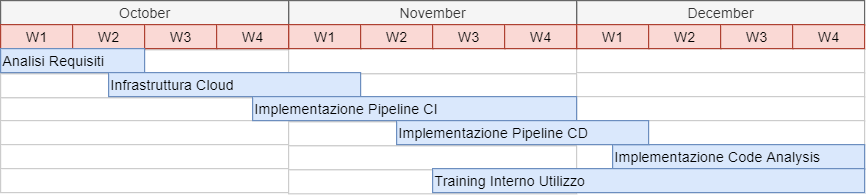
\includegraphics[width=\textwidth]{sphere_gantt}
            		\caption{Project Work Gantt}
            		\label{fig:sphere_gantt}
        	    \end{figure}
    	
    		\subsection*{Prodotti Finali}
    		
    			I prodotti del project work saranno i seguenti:
    			\begin{itemize}
    				\item Analisi dei Requisiti per i processi da implementare;
    				\item Pipeline di Continuous Integration per i servizi di Backend e Mobile;
    				\item Pipeline di Continuous Delivery per i servizi di Backend (Docker Containers);
    				\item Quality Assurance Gates basati sulla analisi dei test e del codice con tools dedicati;
    				\item Infrastruttura basata su Amazon Web Services (Risorse Cloud, VMs) per gestire i processi descritti.
    			\end{itemize}

\end{document}